\documentclass[12pt,nonotes]{beamer}

\usepackage[utf8]{inputenc}

\usetheme{metropolis}
% \usetheme[usetitleprogressbar]{m}
\setbeamertemplate{navigation symbols}{}
%\setbeamertemplate{caption}{\raggedright\insertcaption\par}
%\setbeameroption{show notes}

\newenvironment{changemargin}[2]{%
	\begin{list}{}{%
			\setlength{\topsep}{-1pt}%
			\setlength{\leftmargin}{#1}%
			\setlength{\rightmargin}{#2}%
			\setlength{\listparindent}{\parindent}%
			\setlength{\itemindent}{\parindent}%
			\setlength{\parsep}{\parskip}%
		}%
		\item[]}{\end{list}}
 
\newcommand{\fullframeimage}[1]{
	\begin{frame}[plain]
		\begin{changemargin}{-1cm}{-1cm}
			\begin{center}
				\includegraphics[width=\paperwidth,height=\paperheight,keepaspectratio]
				{#1}
			\end{center}
		\end{changemargin}
	\end{frame}
}

\newcommand{\strong}[1]{ {\large \textbf{#1}} }

\setbeamerfont{bibliography
	entry author}{size=\scriptsize,%
	series=\normalfont}
\setbeamerfont{bibliography
	entry title}{size=\scriptsize,%
	series=\bfseries}
\setbeamerfont{bibliography
	entry location}{size=\tiny,%
	series=\normalfont}

\setbeamerfont{bibliography
	item}{size=\scriptsize,%
	series=\normalfont}


\usepackage{multirow}
\usepackage{subfig}
\usepackage{booktabs}
\usepackage{lmodern}
\usepackage{multicol}
\usepackage{graphicx}
\usepackage{multirow}


\usepackage{amsmath}
\usepackage{moresize}
\usepackage{array}
\usepackage{colortbl}
\usepackage{booktabs} 
\usepackage{pgfplotstable} 

\setbeamertemplate{bibliography item}{\insertbiblabel}

%\author{Klaus Schneider$^1$, Cheng Yi$^2$, Beichuan Zhang$^1$, Lixia Zhang$^3$}
\author{Siham Khoussi$^1$, Klaus Schneider$^2$, Damian Coomes$^3$}
\title{NDN Maps}
\subtitle{4th NDN Hackathon}
%\date{March 24, 2017}
\institute{$^1$NIST, $^2$The University of Arizona, $^3$The University of Memphis}

\begin{document}

\frame{\titlepage}


\begin{frame}{Map Application on NDN}

Why use maps over NDN?
\begin{itemize}
\item Exploiting network awareness of locality
\pause
\item Caching \& Offline Navigation
\pause
\item Privacy
\end{itemize}

\pause
Questions:
\begin{itemize}
\item Namespace design?
\pause
\item Local Forwarding Strategy?
\end{itemize}

	
\end{frame}



\begin{frame}{Wireless Ad-hoc Scenario}
\begin{center}
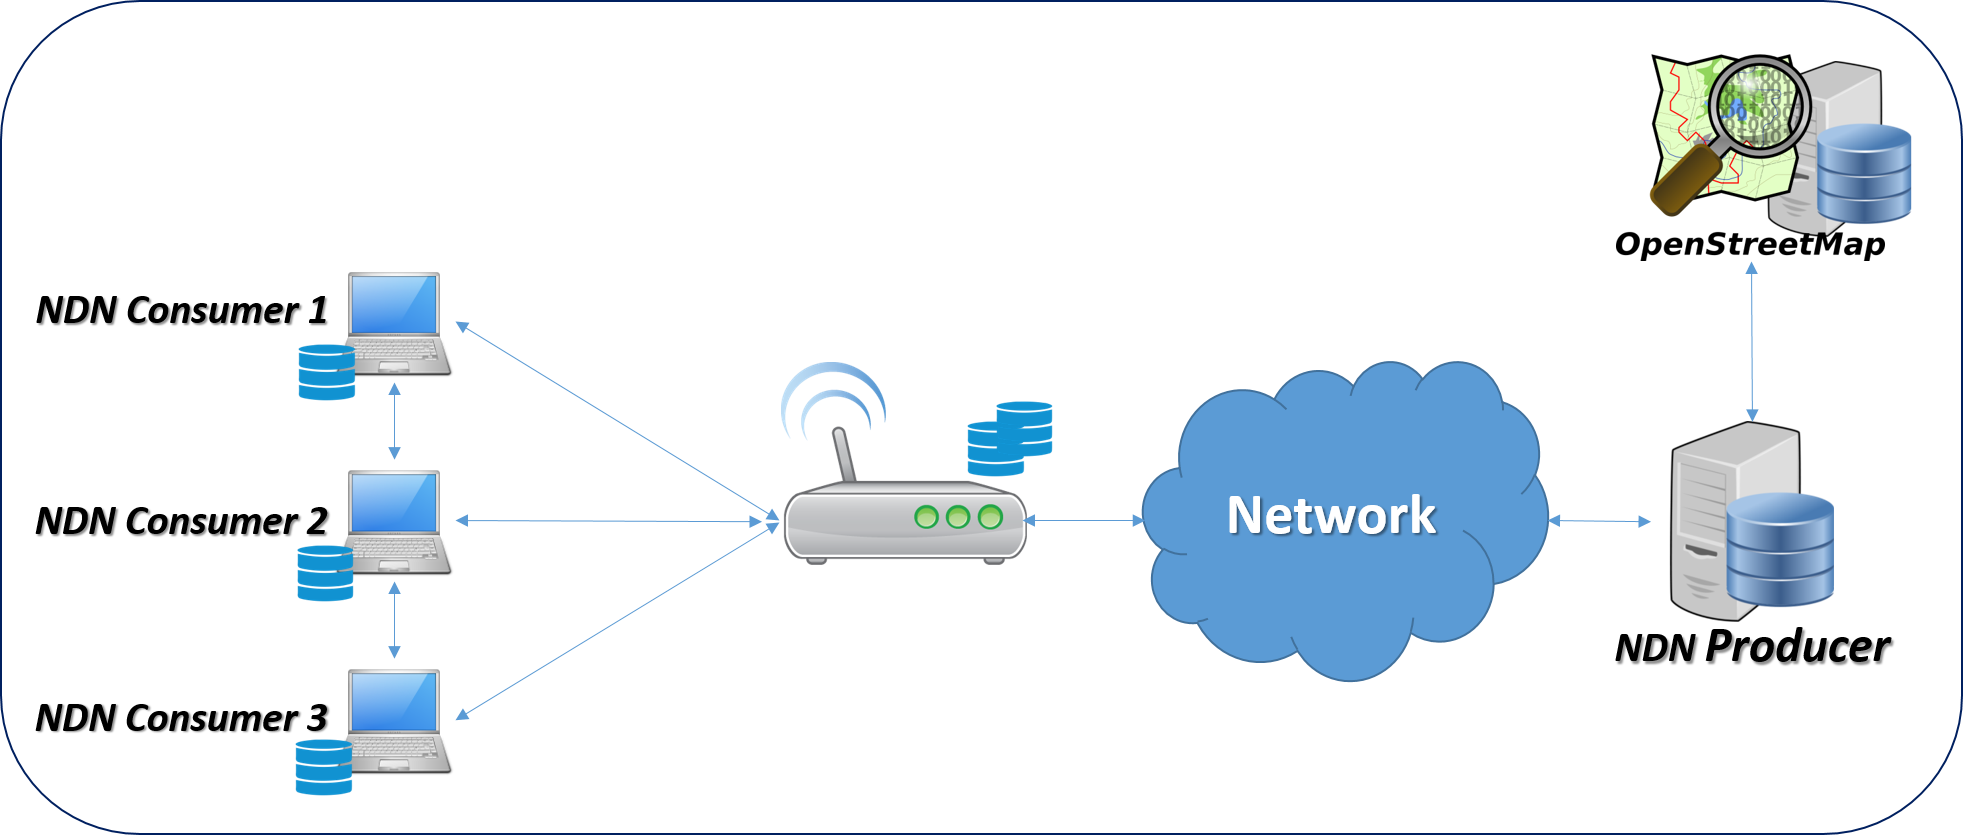
\includegraphics[width=\linewidth]{images/topo2.png}
\end{center}

\end{frame}



\begin{frame}{How OpenStreetMap Works}

\begin{itemize}
\item Tiles: 256x256px (png)
\begin{itemize}
\item Different Zoom Levels (0-19)
\item http://tile.openstreetmap.org/18/129812/85057.png
\item 
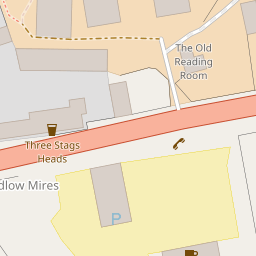
\includegraphics[width=0.25\linewidth]{images/tile.png}
\pause


\end{itemize}
\item Other data: Nodes, Paths (XML, JSON)
\item Why not Google Maps? No access to raw data
\end{itemize}
\pause

Better Namespace?
\begin{itemize}
\item /maps/$Z_0$/$Z_1$/\ldots/$Z_n$
\item $Z_i$ = \{ 0, 1, 2, 3 \}
\end{itemize}
\end{frame}


\begin{frame}{Namespace Example: /maps/0/1/2}
\begin{center}
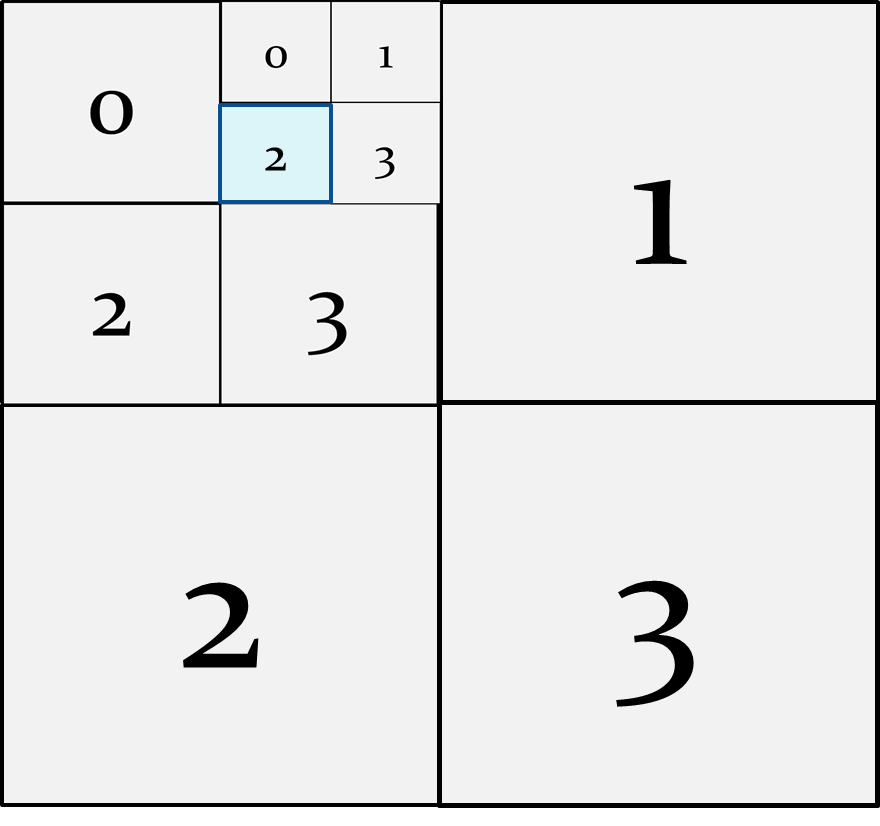
\includegraphics[width=0.75\linewidth]{images/square.png}
\end{center}

\end{frame}



\begin{frame}{Implementation}
\begin{center}
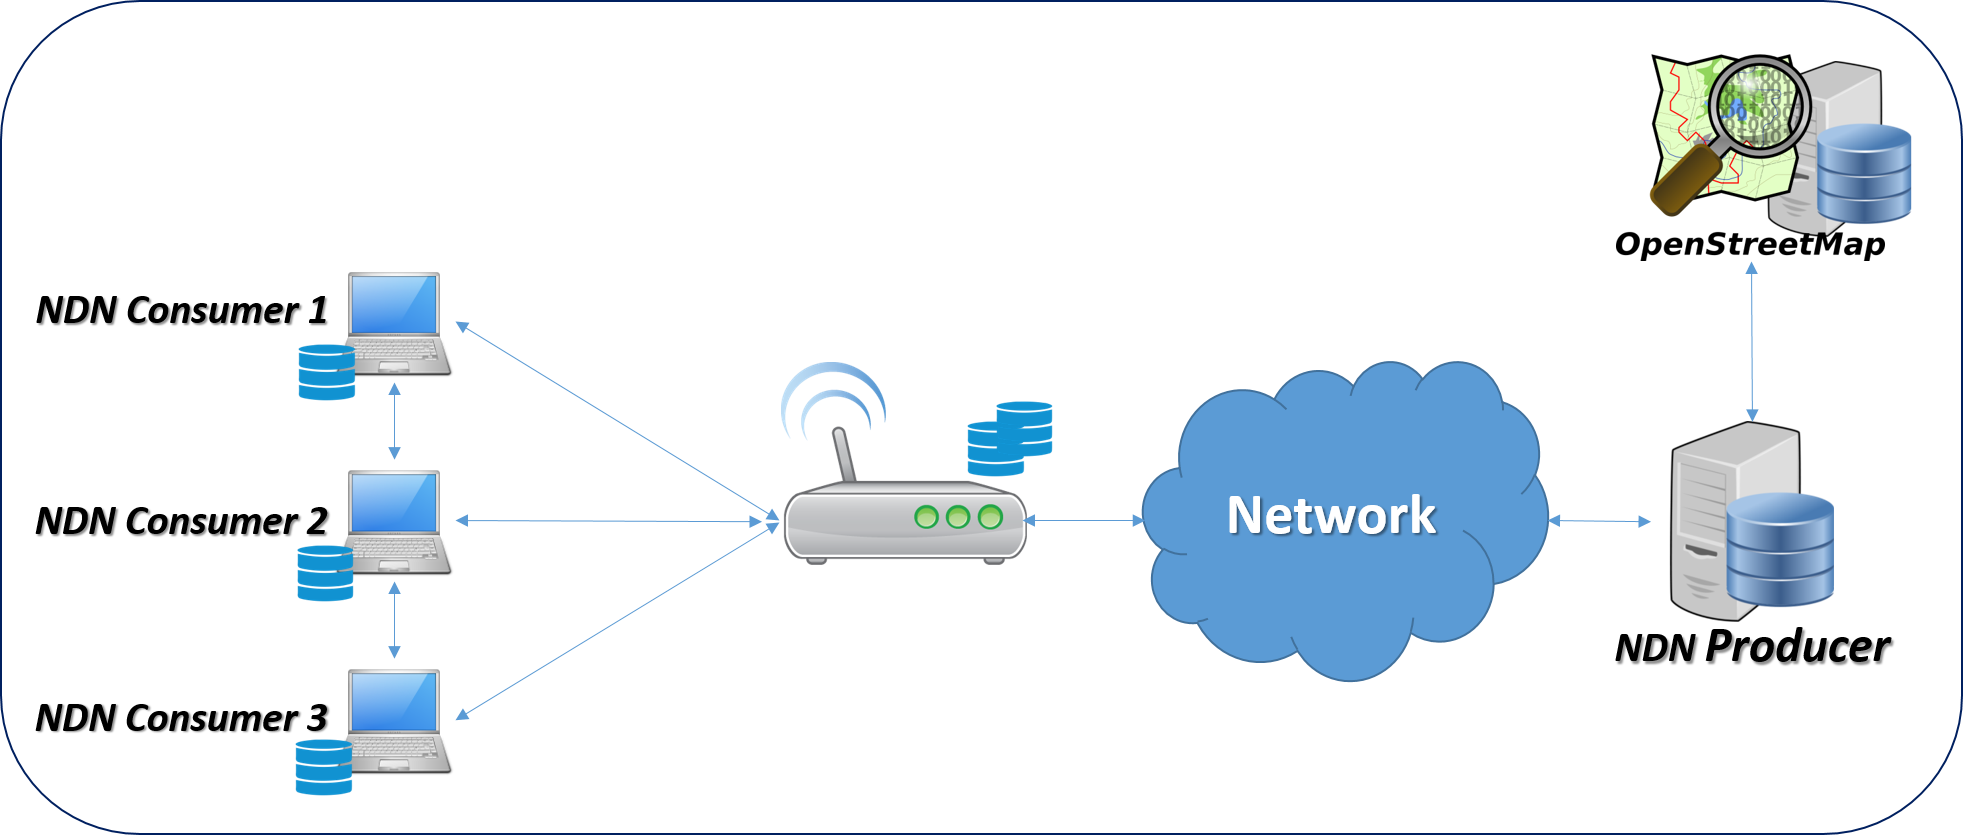
\includegraphics[width=\linewidth]{images/topo2.png}
\end{center}
\end{frame}



\begin{frame}{Implementation}
	
Producer: Fetch data from OSM on demand
\begin{itemize}
\item Map into NDN namespace
\item NDN Java Library
\end{itemize}
\pause

Consumer: Integrate OSM Display Framework with NDN
\begin{itemize}
\item Still work in progress :) 
\end{itemize}

\end{frame}


\begin{frame}{Conclusions}
	
Maps interesting application for NDN
\begin{itemize}
\item Content-awareness of Network Layer
\item Exploiting Locality 
\item Caching \& Offline Use
\end{itemize}

\pause
Future Work:
\begin{itemize}
\item Finishing the Code
\item Navigation
\end{itemize}
	

\end{frame}


%% Last slide
\begin{frame}
	\frametitle{The End}
%	\vspace{1cm}
	{\LARGE Thank you for
		your attention!\\
		\vspace*{2em}
		Questions?
	}
%	\vspace{1.5cm}  
%	\begin{flushright}  
%		Klaus Schneider \\ \footnotesize{\url{klaus@cs.arizona.edu}}
%	\end{flushright}
\end{frame}




%\input{content/oldcontent}

%\begin{frame}[allowframebreaks]{References}
%\scriptsize
%%	\nocite*
%\bibliographystyle{plain} %%% alpha
%%\bibliography{content/bib.bib}
%\bibliography{content/bib_techreport.bib}
%\end{frame}

\end{document}

